\begin{frame}{Recap: Black-Box Testing \deutschertitel{Funktionstest}}
	\begin{mycolumns}[widths={40}]
		\begin{note}{Motivation \mysource{\ludewiglichter}}
			\begin{itemize}
				\setlength\itemsep{.1em}
				\item source code not always available (e.g., outsourced components, obfuscated code)
				%\item specific test cases derived from logical ones using arbitrary values
				%\item specification not incorporated so far (only for expected results)
				%\item invalid inputs not tested
				\item errors are not equally distributed
			\end{itemize}
		\end{note}
		\pause
		\begin{definition}{Black-Box Testing \mysource{\ludewiglichter}}
			\begin{itemize}
				\setlength\itemsep{.1em}
				\item test-case design based on specification
				\item source code and its inner structure is ignored (assumed as a black-box)
			\end{itemize}
		\end{definition}
	\mynextcolumn
		\pause
		\begin{note}{Sample Configuration $\neq$ Test Case}
			\begin{itemize}
				\item test case: concrete inputs and expected outputs for a program
				\item sample configuration: selection of features to derive the program
				\item both needed when testing product lines
				\item often confused in the literature
				\item test case derivation
					\begin{itemize}
						\item out of scope here % TODO add pointers to literature
						\item global tests (i.e., identical for all configurations)
						\item product-line implementation technique used to automatically derive configuration-specific tests \mysource{\lectureprocess}
					\end{itemize}
				\item on next slides: idea of black-box testing applied to derive sample configuration
			\end{itemize}
		\end{note}
	\end{mycolumns}
\end{frame}

\subsection{Pairwise Interaction Testing}
\begin{frame}{\myframetitle{} \deutschertitel{Paarweises Interaktionstesten}}
	\begin{mycolumns}
		\begin{example}{Configurations with the Interaction Get $\wedge$ Put}
			\footnotesize
			\begin{mycolumns}[animation=none,widths={55,45}]
				$\{C,G,W\}$\\
				$\{C,P,W\}$\\
				\emph{$\{C,G,P,W\}$}\\
				$\{C,D,W\}$\\
				$\{C,G,D,W\}$\\
				$\{C,P,D,W\}$\\
				\emph{$\{C,G,P,D,W\}$}\\
				$\{C,P,T,W\}$\\
				\emph{$\{C,G,P,T,W\}$}\\
				$\{C,D,T,W\}$\\
				$\{C,G,D,T,W\}$\\
				$\{C,P,D,T,W\}$\\
				\emph{$\{C,G,P,D,T,W\}$}
			\mynextcolumn
				$\{C,G,L\}$\\
				$\{C,P,L\}$\\
				\emph{$\{C,G,P,L\}$}\\
				$\{C,D,L\}$\\
				$\{C,G,D,L\}$\\
				$\{C,P,D,L\}$\\
				\emph{$\{C,G,P,D,L\}$}\\
				$\{C,P,T,L\}$\\
				\emph{$\{C,G,P,T,L\}$}\\
				$\{C,D,T,L\}$\\
				$\{C,G,D,T,L\}$\\
				$\{C,P,D,T,L\}$\\
				\emph{$\{C,G,P,D,T,L\}$}
			\end{mycolumns}
		\end{example}
		\pause
		\begin{definition}{Pairwise Interaction Testing}
			\begin{itemize}
				\setlength\itemsep{.5em}
				\item create a sample $S \subseteq C$, in which every pairwise interaction is covered by at least one configuration %(all valid configurations $C$)
				\item test every configuration in $S$
			\end{itemize}
		\end{definition}
	\mynextcolumn
		\pause
		\begin{note}{Discussion}
			\begin{itemize}
				\setlength\itemsep{.4em}
				\item applicable to large product lines
				\item reduced redundant effort compared to\\testing all configurations
				\item full coverage guarantee\\(opposed to random configurations)
				\vspace*{1ex}
				\item still requires good test cases (program inputs)
				\item hard to compute small sample sets
			\end{itemize}
		\end{note}
		\pause
		\begin{definition}{Pairwise Combinations}
			\begin{itemize}
				\setlength\itemsep{.5em}
				\item four combinations between $A$ and $B$
				\begin{itemize}
					\item both selected: $A \wedge B$
					\item one selected: $\neg A \wedge B$ and $A \wedge \neg B$
					\item none selected: $\neg A \wedge \neg B$
				\end{itemize}
				\end{itemize}
		\end{definition}
	\end{mycolumns}
\end{frame}

\newcommand{\pair}[2]{$#1 \wedge #2$ & $#1 \wedge \neg #2$ & $\neg #1 \wedge #2$ & $\neg #1 \wedge \neg #2$\\}
\newcommand{\redandgray}[1]{\only<#1-| handout:#1->{\color{black}}\only<#1| handout:#1>{\color{blue}}}
\newcommand{\epair}[6]{
	{\redandgray{#3}$#1 \wedge #2$} & 
	{\redandgray{#4}$#1 \wedge \neg #2$} & 
	{\redandgray{#5}$\neg #1 \wedge #2$} & 
	{\redandgray{#6}$\neg #1 \wedge \neg #2$}\\
}

\begin{frame}{Pairwise Coverage \deutschertitel{Paarweise Überdeckung}}
	\begin{mycolumns}[animation=none]
		\centering
		\alt<1>{\featureDiagramConfigurableDatabase}{%
		\alt<2>{\featureDiagramConfigurableDatabaseNoAbstract}
		{\featureDiagramConfigurableDatabaseNoAbstractNoCore}}

		\pause
		\begin{definition}{Interactions to Cover}
			\begin{itemize}
				\setlength\itemsep{.5em}
				\item<2-> exclude abstract features (e.g., $API$, $OS$)
				\item<3-> exclude features contained in every configuration (e.g., $C$)
				\vspace*{1ex}
				\item<4-> exclude invalid combinations (e.g., $W \wedge L$)
			\end{itemize}
			% TODO \todo{add formal definitions based on \lecturemodeling}
		\end{definition}
	\mynextcolumn
		\vspace{-10mm}
		\pause\pause
		\begin{example}{Pairwise Interactions}
			\centering\footnotesize\color{lightgray}
			\begin{tabular}{llll}
				\epair{G}{P}{7}{6}{5}{10}
				\epair{G}{D}{6}{7}{5}{9}
				\epair{G}{T}{7}{6}{5}{9}
				\epair{G}{W}{8}{6}{5}{10}
				\epair{G}{L}{6}{8}{10}{5}
				\epair{P}{D}{5}{7}{6}{8}
				\epair{P}{T}{5}{9}{10}{6}
				\epair{P}{W}{5}{7}{8}{6}
				\epair{P}{L}{7}{5}{6}{8}
				\epair{D}{T}{5}{6}{7}{8}
				\epair{D}{W}{5}{6}{8}{7}
				\epair{D}{L}{6}{5}{7}{8}
				\epair{T}{W}{5}{7}{8}{6}
				\epair{T}{L}{7}{5}{6}{8}
				& {\redandgray{5}$W \wedge \neg L$} & {\redandgray{6}$\neg W \wedge L$} & \\
			\end{tabular} 
		\end{example}
		\begin{example}{Pairwise Coverage with Six Configurations}
			\footnotesize\color{lightgray}
			{\redandgray{5}$\{C,P,D,T,W\}$}\\
			{\redandgray{6}$\{C,G,D,L\}$}\\
			{\redandgray{7}$\{C,G,P,T,L\}$}\\
			{\redandgray{8}$\{C,G,W\}$}\\
			{\redandgray{9}$\{C,P,W\}$}\\
			{\redandgray{10}$\{C,D,T,L\}$}\\
		\end{example}
	\end{mycolumns}
\end{frame}
% TODO use different colors for the different configurations (instead of separate handouts) + animation showing all pairs in the first place

\subsection{T-Wise Interaction Testing}
\begin{frame}{\myframetitle{}}
	\begin{mycolumns}[widths={60,38}]
		\begin{definition}{T-Wise Interaction Testing}
			\begin{itemize}
				\setlength\itemsep{.5em}
				\item generalization of pairwise interaction testing
				\item t-wise coverage: every t-wise interaction is covered by at least one configuration in the sample
				\item $t=1$: every feature is selected and also deselected
				\item $t=2$: pairwise interaction coverage
				\item $t=3$: every valid combination of three features covered
			\end{itemize}
		\end{definition}
	\mynextcolumn
		\begin{example}{{$t=3$ Interactions}}
			for the features $G$, $P$, and $D$:

			\begin{mycolumns}[animation=none]
				$G \wedge P \wedge D$\\
				$G \wedge P \wedge \neg D$\\
				$G \wedge \neg P \wedge D$\\
				$G \wedge \neg P \wedge \neg D$
			\mynextcolumn
				$\neg G \wedge P \wedge D$\\
				$\neg G \wedge P \wedge \neg D$\\
				$\neg G \wedge \neg P \wedge D$\\
				$\neg G \wedge \neg P \wedge \neg D$
			\end{mycolumns}
		\end{example}
	\end{mycolumns}
\end{frame}

\subsection{Algorithms for Combinatorial Interaction Testing}
\begin{frame}{\myframetitle{} \deutschertitel{Algorithmen für kombinatorisches Interaktionstesten}}
	\begin{mycolumns}[widths={63}]
		\begin{definition}{A Greedy Algorithm}
			idea: select configuration that cover most missing interactions in each step
			\begin{enumerate}
				\item randomly choose first configuration
				\item find next optimal configuration
				\item repeat step 2 until all interactions are covered
			\end{enumerate}
		\end{definition}
		\pause
		\begin{note}{Challenges and Optimizations}
			\begin{itemize}
				\item non-deterministic: different sample for each run (cf.\ Step~1)
				\begin{itemize}
					\item starting with all-yes-config? $\Rightarrow$ covers more code
				\end{itemize}
				\item iterating all valid configurations does not scale (cf.\ Step~2)
				\item greedy strategy: optimal configuration in each step does not guarantee optimal sample
			\end{itemize}
		\end{note}
	\mynextcolumn
		\pause
		\begin{definition}{ICPL\mysource{\icpl}}
			\begin{itemize}
				\item widespread greedy algorithm
				\item iterates over all interactions
				\begin{itemize}
					\item identifies core and dead features early
					\item identifies invalid and already covered interactions
					\item utilizes parallelization
				\end{itemize}
				\item incrementally increases $t$ up to desired value
				\item performance shown on next slides
			\end{itemize}
		\end{definition}
	\end{mycolumns}
\end{frame}

\subsection{Efficiency of Combinatorial Interaction Testing}
%\subsection{Combinatorial Interaction Testing with ICPL}
\begin{frame}{\myframetitle{} \deutschertitel{Algorithmen für kombinatorisches Interaktionstesten} \mytitlesource{\icpl}}
	\begin{exampletight}{Assumption: All Features are Optional}
		\centering\footnotesize\featureDiagramEightOptionalFeatures
	\end{exampletight}

	\pause
	\begin{mycolumns}
		\begin{exampletight}{Number of Configurations in Pairwise Sample}
			\includegraphics[width=\linewidth,page=4]{cit-plots}
		\end{exampletight}
	\mynextcolumn
		\pause
		\begin{exampletight}{Number of Configurations in T-Wise Sample}
			\includegraphics[width=\linewidth,page=5]{cit-plots}
		\end{exampletight}
	\end{mycolumns}
\end{frame}

\begin{frame}{\myframetitle{} \mytitlesource{\icpl}}
	\begin{mycolumns}[forget]
		\begin{exampletight}{Time in Minutes to Compute Sample}
			\includegraphics[width=\linewidth,page=2]{cit-plots}

			\begin{itemize}
				\setlength\itemsep{.5em}
				\item about 9h for Linux
				\item 480 configuration in pairwise sample
			\end{itemize}
		\end{exampletight}
	\mynextcolumn
		\begin{exampletight}{Number of Configurations in Sample}
			\includegraphics[width=\linewidth,page=3]{cit-plots}

			\begin{itemize}
				\setlength\itemsep{.5em}
				\item Linux kernel v2.6.28.6 (February 2009)
				\item 6,888 features
				\item 187,193 clauses in conjunctive normal form
			\end{itemize}
		\end{exampletight}
	\end{mycolumns}
\end{frame}

% TODO distinguish testing efficiency and sampling efficiency

\subsection{Effectiveness of Combinatorial Interaction Testing}
\begin{frame}{\myframetitle{}}
	\begin{mycolumns}[forget]
		\begin{exampletight}{Effectiveness of Interaction Testing \mysource{\href{https://ieeexplore.ieee.org/document/1321063}{Kuhn et al.\ 2004}}}
			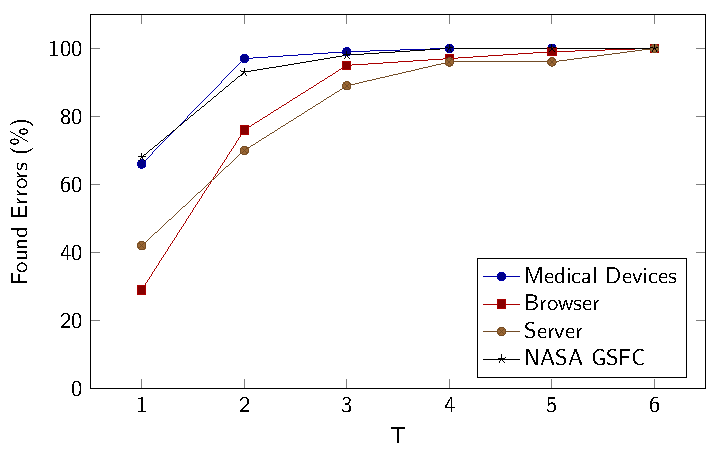
\includegraphics[width=\linewidth,page=1]{cit-plots}
		\end{exampletight}
	\mynextcolumn
		\begin{note}{Trade-Off}
			large t: high coverage (more effective)
			
			small t: low testing effort (more efficient)
		\end{note}
	\end{mycolumns}
\end{frame}
